% par Razieh Pourhasan
\newpage\section{Applications aux séries chronologiques} \label{Section:5}
%\subsection{Application en finance}
Dans cette section, les valeurs aberrantes et les anomalies dans les séries chronologiques sont brièvement examinées. Une série chronologique est un ensemble séquentiel de valeurs suivies sur une durée donnée. R fournit de nombreux progiciels avec différentes approches pour détecter les valeurs aberrantes et les anomalies dans les séries temporelles. Ici, deux des plus couramment utilisées sont introduites et appliquées à une série chronologique de données. \subsection{Outliers et anomalies dans les séries temporelles} \textbf{Les valeurs aberrantes dans les séries chronologiques} sont souvent des changements soudains dans la dynamique des données qui peuvent être temporaires ou permanents. Ces changements sont généralement incohérents avec le reste de la série et ne peuvent pas être expliqués par les modèles de séries chronologiques standard. S'ils ne sont pas traités, ils ont un impact sur l'analyse comme la sélection du modèle et l'estimation des paramètres. Par conséquent, ils ont une incidence sur la puissance de prévision du modèle ajusté. Il est donc important de détecter et de traiter les valeurs aberrantes dans les séries chronologiques avant d'ajuster un modèle. \par valeurs aberrantes qui ne modifient que le niveau moyen de la série sont dites déterministes. Une procédure simple pour détecter les valeurs aberrantes déterministes dans les séries chronologiques consiste à comparer un modèle de série chronologique sans valeurs aberrantes à un autre modèle qui comprend des valeurs aberrantes \cite{tsay}. L'estimation de l'effet du traitement des valeurs aberrantes est alors donnée par les différences entre les modèles. \par En général, la détection des valeurs aberrantes dans les séries chronologiques appliquées consiste à déterminer l'emplacement, le type et l'ampleur de toute valeur aberrante existante. Il existe plusieurs types de valeurs aberrantes, comme indiqué ci-dessous : 
\begin{itemize}[noitemsep]
\item \textbf{Additif aberrant (AO)} est un changement brutal pour une seule valeur observée. Une telle valeur aberrante n'a aucun effet sur les observations ultérieures. Elle est appelée \textbf{valeur aberrante additive saisonnière} lorsqu'une valeur aberrante additive apparaît de façon répétée à intervalles réguliers.
\item \textbf{L'innovation aberrante (IO)} est une innovation inhabituelle\footnote{Les \textit{innovations} dans les séries temporelles sont utilisées de la même manière que les \textit{erreurs} dans l'analyse transversale (comme les MCO). La raison pour laquelle on l'appelle \textit{innovation} est peut-être qu'il apporte de nouvelles informations dans les données des séries chronologiques et qu'il est nouveau dans le sens où les observations sont ordonnées dans le temps.} dans le processus de génération qui affecte toutes les observations ultérieures. L'influence des observations aberrantes peut augmenter avec le temps.
\item \textbf{Décalage de niveau La valeur aberrante (LS)} affecte le niveau moyen des observations de sorte que toutes les observations après la valeur aberrante passent à un nouveau niveau. Il est clair que ces observations aberrantes ont un effet permanent sur la série chronologique ; il est donc important de les détecter et de les traiter avant de construire tout modèle de prévision. On l'appelle \textbf{décalage du niveau saisonnier (DSL)} si le décalage du niveau moyen se produit à intervalles réguliers.
\item \textbf{extrémité de changement transitoire (TC)} est semblable à l'aberration du décalage en niveau, mais son effet n'est pas permanent et disparaît plutôt au cours des observations ultérieures. C'est-à-dire que la série chronologique revient à son niveau normal après un décalage transitoire.
\end{itemize}
\par anomalies sont essentiellement les aberrations. Les choses qui se produisent régulièrement dans la série sont des tendances. Cependant, les observations qui ne se produisent pas souvent et qui s'écartent du schéma ou de la tendance régulière dans la série sont des anomalies.
Le reste de cette section est consacré à l'application des packages R, et des fonctions qu'ils contiennent, pour détecter les valeurs aberrantes et les anomalies. 
\subsection{Package R : tsoutliers} Le paquet \verb|tsoutlier| détecte automatiquement les valeurs aberrantes dans les séries temporelles en se basant sur la procédure proposée par Chen et Liu (1998) \cite{chenliu}. Dans cette approche, les effets aberrants sont estimés simultanément à l'aide d'une régression multiple basée sur ARIMA, et les paramètres du modèle et les effets aberrants sont estimés conjointement. \par L'interface principale de la procédure de détection automatique se fait par la fonction \verb|tso(x, types)|, où \verb|x| est un objet de série temporelle et \verb|types| est un vecteur de caractères indiquant le type de valeurs aberrantes à considérer par la procédure. Les cinq types de valeurs aberrantes décrits dans la section précédente peuvent être pris en compte : \verb|AO|, \verb|IO|, \verb|LS|, \verb|LSL| et \verb|TC|. Si \verb|types| n'est pas spécifié, \verb|AO|, \verb|LS| et \verb|TC| seront considérés par défaut. \par \textbf{Exemple : DJ30\footnote{Le DJ30 est composé de 30 actions qui sont censées refléter la performance du marché américain.}.} Les données historiques de toutes les actions actuellement impliquées dans le Dow Jones Industrial Average sont disponibles en ligne sur Kaggle \cite{dj30}. Pour chacune des 30 composantes de l'indice, il y a un fichier CSV nommé par le symbole de l'action (par exemple AAPL pour Apple Inc.). Chaque fichier fournit des données ajustées historiquement à l'échelle du marché (quotidiennement, il y a 5 ans au maximum). Après avoir lu tous les fichiers CSV avec la fonction \verb|read.csv| dans R, le rendement quotidien de clôture de chaque composante a été trié par date et enregistré dans un cadre de données nommé \verb|data|. Le paquet \verb|tsoutliers| a été téléchargé et les valeurs aberrantes pour Apple Inc. ont été identifiées à l'aide de la fonction \verb|tso| :

\begin{lstlisting}[language=R]
tso(ts(data$AAPL), 
       types=c("TC","AO","LS","IO","SLS"))
\end{lstlisting}
La sortie est un type de liste composé de \verb|Coefficients| et \verb|Outliers|. Voici la sortie R pour les valeurs aberrantes des données d'Apple Inc :
\begin{lstlisting}[language=R]
Outliers:
   type  ind time coefhat  tstat
1    TC  159  159   4.040  4.074
2    AO  302  302  -6.116 -4.405
3    AO  305  305   5.735  4.130
4    AO  410  410  -6.571 -4.732
5    TC  473  473  -4.521 -4.560
6    AO  536  536   6.496  4.678
7    AO  666  666   6.098  4.392
8    AO  791  791   6.629  4.774
9    AO 1043 1043   5.891  4.243
10   AO 1109 1109  -6.633 -4.777
11   AO 1144 1144   7.042  5.072
12   AO 1149 1149  -9.961 -7.174
13   AO 1167 1167   6.833  4.921
14   AO 1238 1238  -5.812 -4.186
\end{lstlisting}
Il y a 14 valeurs aberrantes dont deux sont de type \textit{changement transitoire} et les autres sont des valeurs aberrantes \textit{additifs}. Les valeurs aberrantes ont également été illustrées dans la figure~\ref{fig:apoutlier} ; 
\begin{figure}[t]
\centering
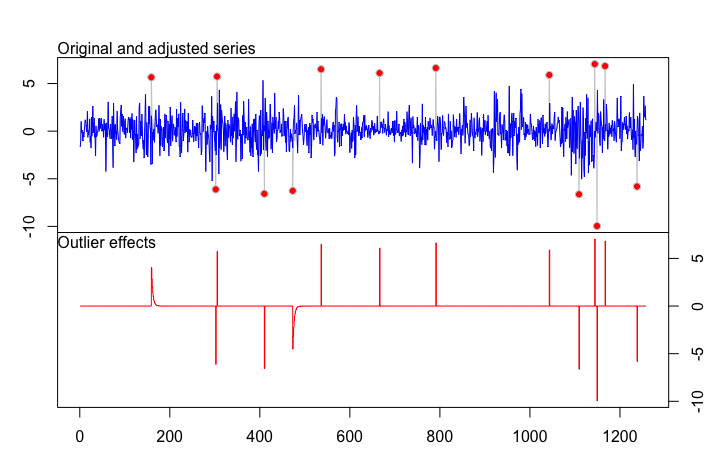
\includegraphics[width=0.30\textwidth]{ADOA/Images/Apoutliers.png}
\caption[\small Détection des valeurs aberrantes pour le rendement quotidien de clôture d'Apple Inc.]{\small Détection des valeurs aberrantes pour le rapport de clôture quotidien d'Apple Inc. L'axe des x est marqué par l'indice de date.}
\hrule\label{fig:apoutlier}
\end{figure}
\afterpage{\FloatBarrier}
Les pics pointus isolés représentent des \textit{additifs aberrants} tandis qu'un pic qui prend quelques périodes pour disparaître représente un \textit{transient changement aberrants}. De plus, notez que l'axe des x a été marqué par l'index heure(date) et non par la date réelle. Cependant, la date réelle peut être facilement obtenue. Dans le code R suivant, la date de chaque sortie a été extraite où la sortie de la fonction \verb|tso| ci-dessus a été enregistrée comme \verb|out_tso| :
\begin{lstlisting}[language=R]
ots=out_tso$outliers
cbind.data.frame(type=ots$type,
                 date=data [ots$ind,1])
\end{lstlisting}
et la sortie est :
\newpage
\begin{lstlisting}[language=R]
   type       date         type       date
1    TC 2015-01-28     8    AO 2017-08-01
2    AO 2015-08-21     9    AO 2018-08-01
3    AO 2015-08-26    10    AO 2018-11-02  
4    AO 2016-01-27    11    AO 2018-12-26
5    TC 2016-04-27    12    AO 2019-01-03
6    AO 2016-07-27    13    AO 2019-01-30
7    AO 2017-02-01    14    AO 2019-05-13
\end{lstlisting}
\subsection{R package : anomalize} La détection d'anomalies est utile à tout spécialiste du marketing pour garder un œil sur la croissance de l'entreprise. Pour le marketing, il est également préférable de faire la détection d'anomalies sur une base quotidienne afin qu'elle aide le spécialiste du marketing à trouver la raison de l'anomalie et aussi à la corriger le plus rapidement possible. Dans cette section, le package \verb|anomalize| est utilisé pour détecter les anomalies dans une série de données temporelles. Le paquet est disponible sur le CRAN, puis la version stable peut être installée directement à partir de là. Cependant, le dernier développement du paquet est disponible sur github. Il est donc recommandé d'installer d'abord le paquet depuis le CRAN afin que les dépendances soient également installées puis de mettre à jour le paquet en utilisant devtools comme indiqué dans le code ci-dessous :
\begin{lstlisting}
install.packages('anomalize')
library(devtools)
install_github("business-science/anomalize")
library(anomalize)
\end{lstlisting}
La fonction \verb|anomalize()| du paquet est utilisée pour détecter les valeurs aberrantes dans une distribution sans tendance ni saisonnalité en utilisant \verb|tidyverse|\footnote{Ce paquet doit être installé aussi.}. Le retour a trois colonnes : "remainder-l1" (limite inférieure pour les anomalies), "remainder-l2" (limite supérieure pour les anomalies), et "anomalie" (Oui/Non). Le premier argument de la fonction est \verb|data| qui est un objet \verb|tibble| ou \verb|tbl_time|. Le deuxième argument \verb|target| est une colonne à laquelle appliquer la fonction, et \verb|method| est la méthode de détection d'anomalie qui peut être une de "iqr" ou "gesd". 
\par La méthode \textbf{IQR} (Intervalle de quartile intérieur) prend une distribution et utilise l'intervalle de quartile intérieur de 25\% et 75\% pour établir la distribution du reste. Les limites sont fixées par défaut à un facteur de 3X au-dessus et au-dessous de l'intervalle de quartile intérieur, et tout reste au-delà des limites est considéré comme une anomalie. Le paramètre alpha ajuste le facteur 3X. Par défaut, alpha = 0,05 pour des raisons de cohérence avec la méthode GESD. Un alpha = 0,025, donne un facteur de 6X, ce qui élargit les limites et rend plus difficile de considérer les données comme une anomalie. Inversement, un alpha = 0,10 contracte les limites à un facteur de 1,5X, ce qui rend plus facile l'identification d'une anomalie dans les données. La méthode IQR ne dépend d'aucune boucle et est donc plus rapide et plus facile à mettre à l'échelle que la méthode GESD. Cependant, elle peut ne pas être aussi précise dans la détection des anomalies puisque les anomalies à fort effet de levier peuvent fausser la ligne centrale (médiane) de l'IQR.
\par La méthode \textbf{GESD} (Generlized Extreme Studentized Deviate Test) élimine progressivement les valeurs aberrantes à l'aide d'un T-Test de Student comparant la statistique du test à une valeur critique. Chaque fois qu'une valeur aberrante est éliminée, la statistique du test est mise à jour. Une fois que la statistique du test tombe en dessous de la valeur critique, toutes les valeurs aberrantes sont considérées comme supprimées. Comme cette méthode implique une mise à jour continue via une boucle, elle est plus lente que la méthode IQR. Cependant, elle tend à être la méthode la plus performante pour l'élimination des valeurs aberrantes. Les arguments restants dans \verb|anomalize()| sont \verb|alpha|, 
\verb|max_anoms| et \verb|verbose| ; le paramètre \verb|alpha| qui est utilisé dans la méthode IQR contrôle la largeur de la plage "normale". Les valeurs inférieures sont plus prudentes, tandis que les valeurs supérieures sont moins susceptibles de classer incorrectement les observations " normales ". \verb|max_anoms| est le pourcentage maximum d'anomalies pouvant être identifiées et \verb|verbose| est un booléen. Si VRAI, retournera une liste contenant des informations utiles sur les anomalies. Si FALSE, renvoie simplement les données développées avec les anomalies et les limites inférieure (l1) et supérieure (l2). \par \textbf{Exemple DJ30-continue.} dans la section précédente, la fonction \verb|tsoutliers| a été utilisée pour détecter les valeurs aberrantes du rendement quotidien de clôture pour l'une des composantes de la DJ30, c'est-à-dire Apple Inc. Une alternative serait la détection d'anomalie à l'aide de \verb|anomalize| qui peut être effectuée à l'aide du code R suivant :

\begin{lstlisting}
data_tb=data %>% as.tibble()
data_tb %>% 
  time_decompose(AAPL,
                 method="stl",
                 frequency=10,
                 trend="auto") %>%
  anomalize(remainder,
            method="gesd",
            alpha=0.05,
            max_anoms=0.2) %>%
  plot_anomaly_decomposition()
\end{lstlisting}
La sortie est illustrée dans la Figure~\ref{fig:apanomalies}.
\begin{figure}[t]
\centering
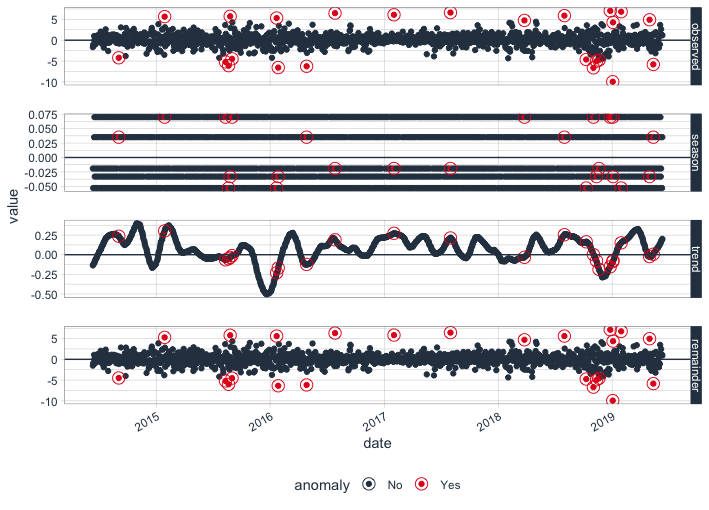
\includegraphics[width=0.5\textwidth]{ADOA/Images/Apanomalies.png}
\caption[\small Détection d'anomalie pour le rapport de clôture quotidien d'Apple Inc.]{\small Détection d'anomalie pour le rapport de clôture quotidien d'Apple Inc.}
\hrule\label{fig:apanomalies}
\end{figure}
\afterpage{\FloatBarrier}
où la placette supérieure est constituée des données globales observées, suivie de la saison et de la tendance, et enfin la placette inférieure permet de détecter les anomalies. Les points rouges dans chaque placette indiquent les anomalies selon la fonction \verb|anomalize|.  Les séries peuvent également être tracées avec des données recomposées selon la fonction \verb|time_recomposed()| à l'aide du code suivant :
\begin{lstlisting}
data_tb %>% 
  time_decompose(AAPL) %>% 
  anomalize(remainder) %>% 
  time_recompose() %>%  
  plot_anomalies(time_recomposed=TRUE,
                 ncol=3,
                 alpha_dots=0.5)
\end{lstlisting}
La sortie est illustrée dans la Figure~\ref{fig:apanomaliesrecomp}.
\begin{figure}[H]
\centering
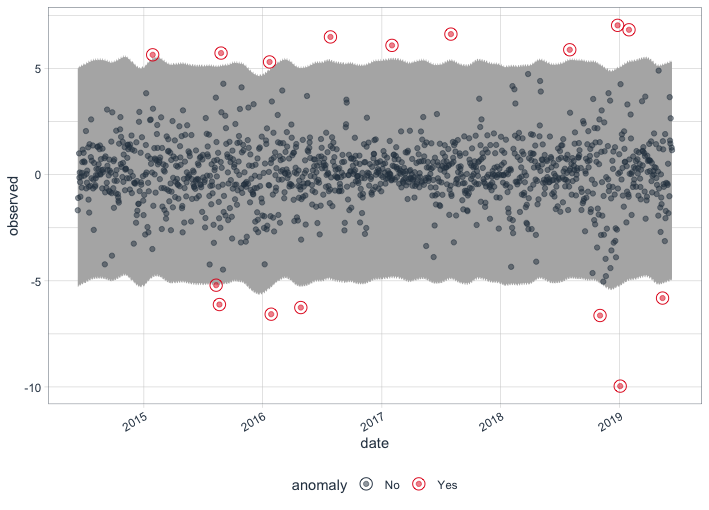
\includegraphics[width=0.5\textwidth]{ADOA/Images/Apanomaliesrecomp.png}
\caption[\small Détection d'anomalie pour le rapport de clôture quotidien d'Apple Inc. avec données recomposées]{\small Détection d'anomalie pour le rapport de clôture quotidien d'Apple Inc. avec données recomposées. La partie grise explique la tendance attendue.}
\hrule\label{fig:apanomaliesrecomp}
\end{figure}
\afterpage{\FloatBarrier}
De plus, les points d'anomalie qui sont indiqués en rouge peuvent être extraits par le code suivant :
\begin{verbatim}
anomalies=data_tb %>% 
  time_decompose(AAPL) %>%  
  anomalize(remainder) %>%  
  time_recompose() %>%  
  filter(anomaly=='Yes')
\end{verbatim}
La sortie est un tableau de temps avec 16 rangées de 10 variables avec \verb|date| et \verb|observed| étant les deux premières variables. Par conséquent, \verb|anomalize| rapporte 16 observations comme anomalies. Rappelez-vous que dans la section précédente, \verb|soutliers| a détecté 14 outliers. Il est intéressant de comparer les dates des observations aberrantes/anomalies pour les données d'Apple Inc. des deux approches. Cela peut être fait avec le code ci-dessous :
\begin{lstlisting}
odates=cbind.data.frame(type=ots$type,
                       date=data[ots$ind,1])
adates=cbind.data.frame(date=anomalies$date,
                observed=anomalies$observed)
left_join(adates,odates,by="date")
\end{lstlisting}
Voici le résultat :
\begin{lstlisting}
        date  observed type
1  2015-01-28    5.653   TC
2  2015-08-11   -5.204 <NA>
3  2015-08-21   -6.116   AO
4  2015-08-26    5.735   AO
5  2016-01-22    5.317 <NA>
6  2016-01-27   -6.571   AO
7  2016-04-27   -6.258   TC
8  2016-07-27    6.496   AO
9  2017-02-01    6.098   AO
10 2017-08-01    6.629   AO
11 2018-08-01    5.891   AO
12 2018-11-02   -6.633   AO
13 2018-12-26    7.042   AO
14 2019-01-03   -9.961   AO
15 2019-01-30    6.833   AO
16 2019-05-13   -5.812   AO
\end{lstlisting}
Il est clair que tous les points qui ont été détectés par \verb|tsoutliers| correspondent à ceux rapportés par \verb|anomalize|. Cependant, \verb|anomalize| détecte deux points supplémentaires qui sont manquants dans la sortie de \verb|tsoutliers|, c'est pourquoi le type n'est pas spécifié pour ces deux points. La comparaison est également illustrée dans la Figure~\ref{fig:comparemethods}.
\begin{figure}[H]
\centering
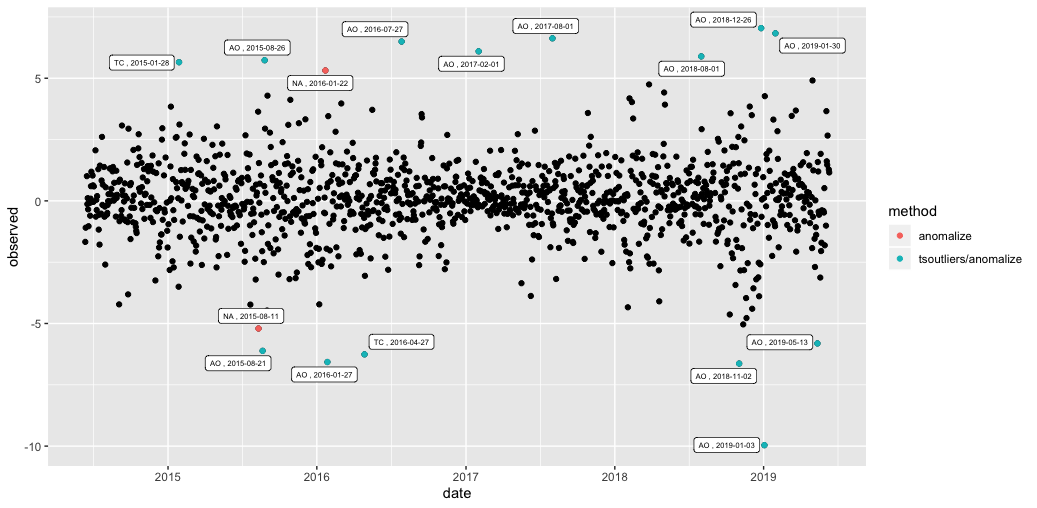
\includegraphics[width=0.5\textwidth]{ADOA/Images/comparemethods.png}
\caption[\small Comparaison de deux méthodes de détection de valeurs aberrantes/anomalies pour le rapport de clôture quotidien d'Apple Inc.] {\small Comparaison de deux méthodes de détection de valeurs aberrantes/anomalies pour le rapport de clôture quotidien d'Apple Inc.}
\hrule\label{fig:comparemethods}
\end{figure}

\afterpage{\FloatBarrier} 

\subsection{Résumé}
Dans de nombreuses disciplines, la détection des valeurs aberrantes est essentielle, mais elle est encore plus importante dans l'analyse marketing où les données sont souvent sous forme de séries chronologiques.  En effet, en marketing, les valeurs aberrantes sont souvent des symptômes visibles de problèmes sous-jacents qui doivent être résolus rapidement. Dans cette section, deux packages R ont été examinés, chacun utilisant une approche différente pour détecter automatiquement les valeurs aberrantes : \verb|soutliers| et \verb|anomalize|, et leurs résultats ont été comparés sur une série temporelle sélectionnée . La définition qui est utilisée dans chaque approche pour détecter les valeurs aberrantes est simple : une valeur aberrante est essentiellement quelque chose qui se produit de façon inattendue ou qui est causé par un événement anormal. Par conséquent, le problème de la détection des valeurs aberrantes consiste à fournir des méthodes permettant de détecter avec précision ces événements \textit{anomalous}. \par Pour les données de séries chronologiques, la détection d'anomalies est généralement effectuée sur les \textbf{retenues} d'une série chronologique où les composantes \textbf{saisonnières} et \textbf{tendance} ont été supprimées ; la première est la présence de variations qui se produisent à des intervalles réguliers spécifiques de moins d'un an, tels que quotidien, hebdomadaire, mensuel ou trimestriel tandis que la seconde est une croissance à plus long terme qui se produit sur de nombreuses observations. Ainsi, la première tâche dans la détection des anomalies est de générer des restes à partir d'une série chronologique. \par Il y a différentes façons de décomposer une série temporelle pour produire des restes comme ARIMA, l'apprentissage machine (régression), la décomposition saisonnière, etc. Le paquet \verb|tsoutliers| utilise ARIMA tandis que \verb|anomalize| utilise la décomposition saisonnière. En général, les techniques d'apprentissage machine à haute performance ne sont pas recommandées pour la détection d'anomalies car le surajustement réduit la différence entre les valeurs observées et ajustées lorsque, comme dans la détection d'anomalies, cette différence est essentielle pour mettre en évidence l'anomalie. En revanche, la décomposition saisonnière est la plus performante pour cette tâche en supprimant les bonnes caractéristiques (c'est-à-dire les composantes saisonnières et tendancielles) tout en préservant les caractéristiques des anomalies dans les restes. \par Comme remarque finale, il y a un autre paquet populaire dans R, c'est-à-dire, \verb|AnomalyDetection| développé par Twitters qui n'est pas examiné ici. Cependant, l'approche qui y est utilisée est similaire à la méthode \textit{GESD} dans \verb|anomalize|. Le lecteur intéressé est invité à essayer ce paquet et les fonctions qu'il contient et à comparer leurs résultats avec les autres fonctions présentées dans cette section.